% (c) 2012 Dimitrios Vrettos - d.vrettos@gmail.com
\section{Esercizi}
\subsection{Esercizi dei singoli paragrafi}
\subsubsection*{10.1 - L'insieme dei monomi}
\begin{esercizio}
\label{ese:10.1}[\Ast]
Individua tra le espressioni letterali di seguito elencate, quelle che sono monomi.
\[E_{1}=35x^{2}+y^{2};\quad E_{2}=-4^{-1}ab^{4}c^{6};\quad E_{3}=\dfrac{4}{x}y^{2};\quad E_{4}=-{\frac{87}{2}}x^{2}z.\]

Per rispondere in modo corretto devo individuare quelle espressioni in
cui compare solamente la \dotfill; pertanto sono monomi \dotfill
\end{esercizio}

\begin{esercizio}
	\label{ese:10.2} %{ese:10.7}
	Individua e sottolinea i monomi tra le seguenti espressioni letterali:
	\[3+ab;\:-2a;\:-\frac{7}{3}ab^2;\:-(\frac{4}{3})^{3};\:a^{2}bc\cdot{\frac{-2}{a^{3}}};\:4a^{-3}b^{2}c^{5};\:-x; 8x^{4}-4x^{2};\:-y\cdot(2x^{4}+6z);\:\frac{abc^{9}}{3+7^{-2}}.\]
\end{esercizio}

\begin{esercizio}
	\label{ese:10.3} %{ese:10.8}
	Nel monomio~$m=-{\frac{5}{2}}a^{3}x^{2}y^{4}z^{8}$ distinguiamo: coefficiente~$=\ldots$,
	parte letterale~$=\ldots$,
	grado complessivo~$=\ldots$,
	il grado della lettera~$x=\ldots$
\end{esercizio}
\begin{esercizio}
\label{ese:10.4}
Scrivi in forma normale i seguenti monomi:
\begin{multicols}{2}
\begin{enumeratea}
 \item $\dfrac{4}{9}ab18c^{3}2^{-2}a^{3}b=\dfrac{\ldots }{\ldots }a^{\ldots}b^{\ldots }c^{\ldots }$;
 \item $-x^{5}\dfrac{1}{9}y^{4}\big(-1+5\big)^{2}y^{7}=\dotfill~$
\end{enumeratea}
\end{multicols}
\end{esercizio}

%\begin{esercizio}
%\label{ese:10.3}
%Nell'insieme
%$M=\big\{-{\frac{34}{5}}a^{3}b\text{,~}3^{2}a^{2}b^{4}\text{,~}\frac{1}{3}ab^{3}\text{,~}a^{3}b\text{,~}-a\text{,~}7a^{2}b^{4}\text{,~}-\frac{1}{3}ab^{3}\text{,~}-89a^{3}b\big\}$,
%determina i sottoinsiemi dei monomi simili e rappresentali con un diagramma di Venn.
%\end{esercizio}

\subsubsection*{10.2 - Valore di un monomio}

\begin{esercizio}
\label{ese:10.5} %{ese:10.3}
Calcola l'area di un triangolo che ha altezza~$h=\np{2,5}$ e base~$b=\frac{3}{4}$.
\end{esercizio}

\begin{esercizio}[\Ast]
	 \label{ese:10.6} %{ese:10.4}
 Calcola il valore dei seguenti monomi in corrispondenza dei valori indicati per ciascuna lettera.

\begin{multicols}{2}
\begin{enumeratea}
 \item $-\frac{2}{9}xz$ per $ x=\frac{1}{2} $, $z=-1$;
 \item $-\frac{8}{5}x^{2}y$ per $ x=-1 $, $y=+10$;
 \item $-\frac{1}{2}a^{2}bc^3$ per $ a=-\frac{1}{2} $, $b=\frac{3}{2},c=-1$;
 \item $\frac{7}{2}a^{3}x^{4}y^2$ per $ a=\frac{1}{2} $, $x=2$, $y=-\frac{1}{2}$;
 \item $\frac{8}{3}abc^2$ per $ a=-3 $, $b=-\frac{1}{3},c=\frac{1}{2}$.
\end{enumeratea}
\end{multicols}
\end{esercizio}


\begin{esercizio}[\Ast]
 \label{ese:10.7} %{ese:10.5}
 Il grado complessivo di un monomio è:

\begin{enumeratea}
 \item l'esponente della prima variabile che compare nel monomio;
 \item la somma di tutti gli esponenti che compaiono sia ai fattori
numerici sia a quelli letterali;
 \item il prodotto degli esponenti delle variabili che compaiono nel monomio;
 \item la somma degli esponenti di tutte le variabili che vi compaiono.
\end{enumeratea}
\end{esercizio}


\begin{esercizio}[\Ast]
 \label{ese:10.8} %{ese:10.6}
Due monomi sono simili se:

\begin{enumeratea}
 \item hanno lo stesso grado;
 \item hanno le stesse variabili;
 \item hanno lo stesso coefficiente;
 \item hanno le stesse variabili con rispettivamente gli stessi esponenti.
\end{enumeratea}
\end{esercizio}
\pagebreak
\begin{esercizio}
 \label{ese:10.9} %{ese:10.10}
Motiva brevemente la verità o falsità delle seguenti proposizioni:
\TabPositions{8.5cm}
\begin{enumeratea}
 \item ``Se due monomi hanno ugual grado allora sono simili''\tab\boxV\quad\boxF\qquad perché\dotfill
 \item ``Se due monomi sono simili allora hanno lo stesso grado''\tab\boxV\quad\boxF\qquad perché\dotfill
\end{enumeratea}
\end{esercizio}

\begin{esercizio}
 \label{ese:10.10} %{ese:10.11}
Quale dei diagrammi di Venn di seguito riportati rappresenta in modo corretto la seguente proposizione: <<alcune espressioni letterali non sono monomi>>.
$L$: insieme delle espressioni letterali, $M$: insieme dei monomi.
\begin{center}
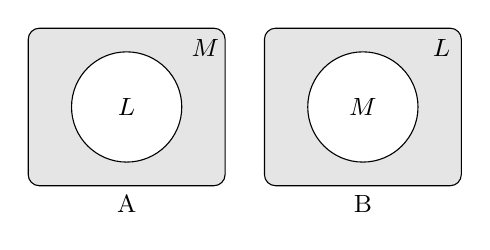
\begin{tikzpicture}[x=5mm, y=5mm,font=\small]
\definecolor{area}{gray}{0.9}
\draw [rounded corners, fill=area] (0,0) rectangle (5,4)  (4.5,3.5)node {$M$}; 
\draw[fill=white] (2.5,2) circle (1.4) node {$L$};
\node[below] at (2.5,0) {A};

\begin{scope}[xshift=30mm]
\draw [rounded corners, fill=area] (0,0) rectangle (5,4)  (4.5,3.5)node {$L$}; 
\draw[fill=white] (2.5,2) circle (1.4) node {$M$};
\node[below] at (2.5,0) {B};
\end{scope}
\end{tikzpicture}
\end{center}
\end{esercizio}

\begin{esercizio}[\Ast]
 \label{ese:10.11} %{ese:10.12}
 Attribuisci il valore di verità alle seguenti proposizioni:
\TabPositions{11.5cm}
\begin{enumeratea}
\item Il valore del monomio~$-a$ è negativo per qualunque $a$ diverso da zero.\tab\boxV\quad\boxF
\item Il valore del monomio~$-a^{2}$ è negativo per qualunque $a$ diverso da zero.\tab\boxV\quad\boxF
\item Il monomio~$b^{6}$ è il cubo di~$b^{2}$.\tab\boxV\quad\boxF
\item L'espressione~$ab^{-1}$ è un monomio.\tab\boxV\quad\boxF
\item Il valore del monomio $ab$ è nullo per~$a = 1$ e $b =-1$.\tab\boxV\quad\boxF
\end{enumeratea}
\end{esercizio}


\subsubsection*{10.3 - Moltiplicazione di due monomi}

\begin{esercizio}[\Ast]
 \label{ese:10.12} %{ese:10.13}
Determina il prodotto dei seguenti monomi.
\begin{multicols}{2}
\begin{enumeratea}
\spazielenx
 \item $\big(-x^{2}y^{4}\big)\cdot \bigg(-{\dfrac{8}{5}}x^{2}y\bigg)$;
 \item $\bigg(-{\dfrac{15}{28}}xy^{3}\bigg)\cdot\bigg(-\dfrac{7}{200}x^{2}y^{2}\bigg)$;
 \item $\big(a^{5}b^{5}y^{2}\big)\cdot\bigg(-\dfrac{8}{5}a^{2}y^{2}b^{3}\bigg)$;
 \item $\np{2,5}ab^{2}\cdot \bigg(-{\dfrac{1}{2}}a^{2}b\bigg)\cdot \np{1,5}a$;
 \item $\bigg(-{\dfrac{2}{9}}xz\bigg)\bigg(-{\dfrac{1}{4}}z^{3}\bigg)(27x)$;
 \item $-8\bigg(\dfrac{1}{4}x\bigg)\bigg(\dfrac{4}{5}x^{3}a^{4}\bigg)$;
 \item $5x^{3}y^{2}\cdot \bigg(-{\dfrac{1}{3}}x^{3}y^{2}\bigg)\cdot \bigg(-{\dfrac{1}{3}}\bigg)$;
 \item $6ab\cdot \bigg(-{\dfrac{1}{3}}a^{2}\bigg)\cdot {\dfrac{1}{2}ab\cdot 4a^{2}}$;
 \item $\bigg(\dfrac{7}{2}a^{3}x^{{4}}y^{2}\bigg)\cdot \bigg(-{\dfrac{8}{21}}ax^{2}y\bigg)$.
\end{enumeratea}
\end{multicols}
\end{esercizio}

%\pagebreak
\begin{esercizio}[\Ast]
 \label{ese:10.13} %{ese:10.14}
Determina il prodotto dei seguenti monomi.
\begin{multicols}{3}
\begin{enumeratea}
\spazielenx
 \item $(-2xy)\cdot (+3ax)$;
 \item $6a(-2ab)\big(-3a^{2}b^{2}\big)$;
 \item $(-1)(-ab)$;
 \item $\np{1,5}a^{2}b\cdot \bigg(-{\dfrac{2}{3}}a^{2}b\bigg)$;
 \item $-{\dfrac{7}{5}}xy^{3}\bigg(-{\dfrac{10}{3}}xy^{2}z\bigg)$;
 \item $-x\big(14x^{2}\big)$.
\end{enumeratea}
\end{multicols}
\end{esercizio}
\pagebreak
\begin{esercizio}[\Ast]
 \label{ese:10.14} %{ese:10.15}
Determina il prodotto delle seguenti coppie di monomi.
\begin{multicols}{3}
\begin{enumeratea}
 \item $\np{1,}\overline{{6}}xa\big(\np{1,2}xy^{2}\big)$;
 \item $\bigg(\dfrac{12}{7}m^{2}n^{3}\bigg)\bigg(-{\dfrac{7}{4}}mn\bigg)$;
 \item $\bigg(-{\dfrac{5}{4}}ax^{2}\bigg)\bigg(\dfrac{3}{10}x^{3}y\bigg)$;
 \item $12ab\bigg(-{\dfrac{1}{2}}a^{3}b^{3}\bigg)$;
 \item $\bigg(-{\dfrac{15}{8}}at^{2}\bigg)\bigg(\dfrac{6}{5}t^{3}x\bigg)$;
 \item $\bigg(\dfrac{12}{4}a^{2}n^{2}\bigg)\bigg(-{\dfrac{7}{4}}ax\bigg)$;
 \item $3ab^2\left(-2a^2b\right)\dfrac{ab}{2}$;
 \item $\dfrac{ab}{4}\left(-2x^2\right)(-2ax)$;
 \item $\dfrac{3}{5}a^4\left({2ab^2}\right)\left(-\dfrac{15}{6a^3b}\right)$.
\end{enumeratea}
\end{multicols}
\end{esercizio}


\begin{esercizio}[\Ast]
 \label{ese:10.15} %{ese:10.16}
In base agli esercizi precedenti puoi concludere che il grado del monomio prodotto è:

\begin{enumeratea}
 \item il prodotto dei gradi dei suoi fattori;
 \item la somma dei gradi dei suoi fattori;
 \item minore del grado di ciascuno dei suoi fattori;
 \item uguale al grado dei suoi fattori.
\end{enumeratea}
\end{esercizio}

\subsubsection*{10.4 - Potenza di un monomio}
\begin{esercizio}[\Ast]
 \label{ese:10.16} %{ese:10.17}
 Esegui le potenze indicate.
\begin{multicols}{2}
\begin{enumeratea}
\spazielenx
 \item $\bigg(-{\dfrac{3}{5}}abx^{3}y^{5}\bigg)^{3}=\dfrac{\ldots }{\ldots}a^{3}b^{3}x^{\ldots }y^{\ldots}$;
 \item $\big(-a^{4}b^{2}\big)^{7}=\ldots$;
 \item $\bigg(-3x^{3}y^{4}z\bigg)^{2}=9x^{6}y^{\ldots }z^{\ldots }$;
 \item $\bigg(\dfrac{1}{2}a^{2}bc^{5}\bigg)^{4}=\dfrac{1}{\ldots}a^{\ldots}b^{\ldots}c^{\ldots}$;
 \item $\big(a^{3}b^{2}\big)^{8}=\ldots$;
 \item $\big(-5ab^{2}c\big)^{3}=\ldots$
\end{enumeratea}
\end{multicols}
\end{esercizio}

\begin{esercizio}[\Ast]
 \label{ese:10.17} %{ese:10.18}
 Esegui le potenze indicate.
\begin{multicols}{3}
\begin{enumeratea}
\spazielenx
 \item $\big(+2ax^{3}y^{2}\big)^{2}$;
 \item $\bigg(-{\dfrac{1}{2}}axy^{2}\bigg)^{3}$;
 \item $\bigg(\dfrac{3}{4}x^{4}y\bigg)^{3}$;
 \item $\bigg(\dfrac{2}{3}xy^{2}\bigg)^{3}$;
 \item $\bigg(-{\dfrac{1}{2}}ab\bigg)^{4}$;
 \item $\bigg(-{\dfrac{3}{2}}a^{5}\bigg)^{2}$.
\end{enumeratea}
\end{multicols}
\end{esercizio}

\begin{esercizio}[\Ast]
 \label{ese:10.18} %{ese:10.19}
 Esegui le operazioni indicate.
\begin{multicols}{2}
\begin{enumeratea}
\spazielenx
 \item $\bigg[\big(-rs^{2}t\big)^{2}\bigg]^{3}$;
 \item $\Bigg[\bigg(-{\dfrac{1}{2}}x^{2}y^{3}\bigg)^{2}\Bigg]^{3}$;
 \item $\Bigg[\bigg(-{\dfrac{3}{2}}a^{2}b^{3}\bigg)^{2}\Bigg]^{2}$;
 \item $\big(-xy\big)^{2}\bigg(-{\dfrac{1}{2}}xy^{2}\bigg)^{3}$;
 \item $-\bigg(\dfrac{3}{2}xy^{2}\bigg)^{0}\cdot\bigg(-{\dfrac{1}{6}}xy\bigg)^{2}$;
 \item $-\bigg(-{\dfrac{1}{3}}x^{3}y^{2}\bigg)^{2}\cdot\bigg(-{\dfrac{1}{3}}\bigg)^{-3}$.
\end{enumeratea}
\end{multicols}
\end{esercizio}
\pagebreak
\begin{esercizio}[\Ast]
 \label{ese:10.19} %{ese:10.20}
 Esegui le operazioni indicate.
\begin{multicols}{2}
\begin{enumeratea}
\spazielenx
 \item $\bigg(\dfrac{2}{3}ab^{2}c\bigg)^{2}\cdot\big(-3ab^{3}\big)^{2}$;
 \item $\Bigg[\bigg(-{\dfrac{1}{2}}a^{2}b\bigg)^{2}\cdot{\dfrac{2}{3}a^{2}b}\Bigg]^{2}$;
 \item $\bigg(\dfrac{2}{3}x\cdot{\dfrac{1}{6}}x\cdot {\dfrac{1}{2}}x\bigg)^{2}\cdot\bigg(-{\dfrac{1}{6}}ab^{2}\bigg)^{2}$.
 \item $\left(-2x^2y^3\right)^2\left(2x^2y\right)^3$;
 \item $\left(-\dfrac{2}{5}xy^3\right)^3\left(\dfrac{5}{18}x^3y^5\right)^2\left(-3xy\right)^3$;
 \item $\left(-\dfrac{2}{3}xy^2\right)^2\left(-\dfrac{4}{9}a^2xy^3\right)^2\left(-\dfrac{3}{4}x^2\right)^3$.
\end{enumeratea}
\end{multicols}
\end{esercizio}

\subsubsection*{10.5 - Divisione di due monomi}
\begin{esercizio}[\Ast]
 \label{ese:10.20} %{ese:10.21}
Esegui le divisioni indicate e poni le condizioni di esistenza~$(\CE)$:
\begin{multicols}{2}
\begin{enumeratea}
\spazielenx
 \item $15b^{8}:\bigg(-{\dfrac{40}{3}}b^{3}\bigg)$;
 \item $\bigg(-{\dfrac{13}{72}}x^{2}y^{5}z^{3}\bigg):\bigg(-{\dfrac{26}{27}}xyz\bigg)$;
 \item $(-a^{7}):(8a^{7})$;
 \item $\bigg(\dfrac{1}{2}a^{3}\bigg):(-4a^{5})$;
 \item $\bigg(-{\dfrac{12}{2}}a^{7}b^{5}c^{2}\bigg):(-18ab^{4}c)$;
 \item $(-34x^{5}y^{2}):(-2yz^{3})$;
 \item $\dfrac{2}{5}a^3b^2:\left(-\dfrac{4}{5}ab^2c^2\right)$;
 \item $\dfrac{9}{5}a^4b^7c^2:\left(-\dfrac{3}{2}a^6b^5c\right)$.
% \item $\dfrac{2}{5}a^2b:\left(-\dfrac{3}{5}ab\right):\dfrac{5}{9}b$.
\end{enumeratea}
\end{multicols}
\end{esercizio}

\begin{esercizio}[\Ast]
 \label{ese:10.21} %{ese:10.22}
Esegui le divisioni indicate e poni le condizioni di esistenza~$(\CE)$:
\begin{multicols}{2}
\begin{enumeratea}
 \item $21a^{3}x^{4}b^{2}:\left(7ax^{2}b\right)$;
 \item $a^{6}:\left(20a^{2}\right)$;
 \item $20ax^{4}y:(2xy)$;
 \item $-72a^{4}b^{2}y^{2}:(-3ab^{2})$.
\end{enumeratea}
\end{multicols}
\end{esercizio}

\begin{esercizio}[\Ast]
 \label{ese:10.22} %{ese:10.23}
Esegui le divisioni indicate e poni le condizioni di esistenza~$(\CE)$:
\begin{multicols}{2}
\begin{enumeratea}
 \item $48a^{5}bx:\left(a^{2}b\right)$;
 \item $\Bigg[-\bigg(-{\dfrac{1}{3}}x^{3}y^{2}\bigg)^{2}:\bigg(-{\dfrac{1}{3}}\bigg)\Bigg]^{2}:(x^{3}y^{2})^{2}$;
 \item $\Bigg[\dfrac{3}{5}x^{4}:\bigg(\dfrac{1}{3}x^{4}\bigg)\Bigg]\cdot\Bigg[x^{4}:\bigg(\dfrac{4}{5}x^{4}\bigg)\Bigg]$;
 \item $\bigg(\dfrac{2}{3}ab^{2}c\bigg)^{2}:(-3ab^{3})$.
\end{enumeratea}
\end{multicols}
\end{esercizio}

\subsubsection*{10.6 - Addizione di due monomi simili}
\begin{esercizio}
 \label{ese:10.23} %{ese:10.24}
Determina la somma dei monomi simili~$8a^{2}b+(-{\frac{2}{3}})a^{2}b+\frac{1}{6}a^{2}b$.

La somma è un monomio \ldots\ldots\ldots agli
addendi; il suo coefficiente è dato da
$8-\frac{2}{3}+\frac{1}{6}=\ldots $, la parte letterale è~$\dotfill~$ Quindi la
somma è~$\dotfill$
\end{esercizio}

\begin{esercizio}
 \label{ese:10.24} %{ese:10.25}
Determina la somma~$2a-3ab-a+17ab+41a$.

I monomi addendi non sono tra loro simili, modifico la scrittura
dell'operazione applicando le proprietà associativa e commutativa
in modo da affiancare i monomi simili:
\[S=2a-3ab-a+17ab+41a=(\ldots\ldots\ldots)+(\ldots\ldots\ldots)=\ldots\ldots\ldots\]
La somma ottenuta non è un \ldots\ldots\ldots\ldots\ldots
\end{esercizio}
\pagebreak
\begin{esercizio}[\Ast]
 \label{ese:10.25} %{ese:10.26}
Esegui la somma algebrica dei seguenti monomi.
\begin{multicols}{3}
\begin{enumeratea}
 \item $6x+2x-3x$;
 \item $-3a+2a-5a$;
 \item $5a^{2}b-3a^{2}b$;
 \item $a^{2}b^{2}-3a^{2}b^{2}$;
 \item $2xy-3xy+xy$;
 \item $2y^{2}-3y^{2}+7y^{2}-4y^{2}$.
\end{enumeratea}
\end{multicols}
\end{esercizio}

\begin{esercizio}[\Ast]
 \label{ese:10.26} %{ese:10.27}
Esegui la somma algebrica dei seguenti monomi.
\begin{multicols}{3}
\begin{enumeratea}
 \item $-2xy^{2}+xy^{2}$;
 \item $-3ax-5ax$;
 \item $5ab-2ab$;
 \item $-3xy^{2}+3xy^{2}$;
 \item $7xy^{3}-2xy^{3}$;
 \item $+2xy^{2}-4xy^{2}$.
\end{enumeratea}
\end{multicols}
\end{esercizio}

\begin{esercizio}[\Ast]
 \label{ese:10.27} %{ese:10.28}
Esegui la somma algebrica dei seguenti monomi.
\begin{multicols}{2}
\begin{enumeratea}
 \item $\dfrac{1}{2}a^{2}-a^{2}$;
 \item $+2xy^{2}-4xy^{2}+xy^{2}$;
 \item $-5x^{2}+3x^{2}$;
 \item $\dfrac{1}{2}a+2a$;
 \item $5a^{2}b+2a^{2}b+a^{2}b-3a^{2}b-a^{2}b$;
 \item $\np{0,1}x-5x-\np{1,2}x+3x$.
\end{enumeratea}
\end{multicols}
\end{esercizio}

\begin{esercizio}[\Ast]
 \label{ese:10.28} %{ese:10.29}
Esegui la somma algebrica dei seguenti monomi.
\begin{multicols}{2}
\begin{enumeratea}
\spazielenx
 \item $\dfrac{1}{4}a^{3}b^{2}-\dfrac{1}{2}a^{3}b^{2}$;
 \item $\dfrac{2}{3}x-\dfrac{2}{5}x-2x+\dfrac{3}{10}x$;
 \item $\dfrac{2}{5}ab-\dfrac{1}{2}ab+\dfrac{27}{2}ab-\dfrac{1}{10}ab-\dfrac{5}{2}ab$;
 \item $-\bigg(-{\dfrac{1}{2}}ax^{2}\bigg)-3ax^{2}$;
 \item $-{\dfrac{9}{2}}xy-(-xy)$;
 \item $2xy^{2}-\dfrac{3}{2}xy^{2}-xy^{2}$.
\end{enumeratea}
\end{multicols}
\end{esercizio}

\begin{esercizio}[\Ast]
 \label{ese:10.29} %{ese:10.30}
Esegui la somma algebrica dei seguenti monomi.
\begin{multicols}{2}
\begin{enumeratea}
\spazielenx
 \item $\dfrac{1}{2}a+2a+(2a-a)-\bigg(3a-\dfrac{1}{2}a\bigg)$;
 \item $6xy^{2}+\dfrac{1}{3}xy^{2}-\dfrac{1}{4}xy^{2}-6xy^{2}$;
 \item $\dfrac{1}{2}xy^{2}+\dfrac{3}{2}xy^{2}$;
 \item $\bigg(\dfrac{2}{3}a+a\bigg)-\bigg(\dfrac{2}{3}a-a\bigg)$;
 \item $5ab-2ab+(-ab)-(+2ab)+ab$;
 \item $\np{-1,2}x^{2}+\np{0,1}x^{2}+(-5x)^{2}-(-25x)^{2}$.
\end{enumeratea}
\end{multicols}

\end{esercizio}

\begin{esercizio}[\Ast]
 \label{ese:10.30} %{ese:10.31}
Esegui le operazioni indicate.
\begin{multicols}{2}
\begin{enumeratea}
\spazielenx
 \item $6ab-\dfrac{1}{3}a^{2}+\dfrac{1}{2}ab+4a^{2}$;
 \item $\bigg(\dfrac{1}{4}x^{2}-\dfrac{3}{4}x^{2}+x^{2}\bigg)-\bigg(-{\dfrac{1}{3}}x^{2}+\dfrac{1}{2}x^{2}\bigg)$;
 \item $-{\dfrac{4}{3}}a^{2}b^{3}-2a^{2}b^{3}+\dfrac{1}{3}a^{2}b^{3}-a^{2}b^{3}$;
 \item $\big(-xy\big)^{2}\bigg(-{\dfrac{1}{2}}xy^{2}\bigg)+\dfrac{3}{2}xy^{2}\bigg(-{\dfrac{1}{6}}xy\bigg)^{2}$.
\end{enumeratea}
\end{multicols}
\end{esercizio}

\begin{esercizio}[\Ast]
 \label{ese:10.31} %{ese:10.32}
Esegui la somma algebrica dei seguenti monomi.

\begin{enumeratea}
\spazielenx
 \item $\dfrac{1}{2}x^{2}-2x^{2}-\bigg(-{\dfrac{1}{2}}x^{2}+\dfrac{3}{4}x^{2}-2x^{2}-\dfrac{3}{5}x^{2}\bigg)$;
 \item $5x^{3}y^{2}+\bigg(-{\dfrac{1}{3}}x^{3}y^{2}\bigg)+\bigg(-{\dfrac{1}{3}}\bigg)-\big(x^{3}y^{2}\big)+\bigg(-{\dfrac{1}{4}}x^{3}y^{2}\bigg)-\bigg(-{\dfrac{1}{3}}\bigg)$;
 \item $\bigg(2xy^{2}-\dfrac{3}{2}xy^{2}\bigg)-\big(xy^{2}+2xy^{2}-4xy^{2}\big)+\bigg(xy^{2}+\dfrac{1}{2}xy^{2}\bigg)$.
\end{enumeratea}
\end{esercizio}

\subsubsection*{10.7 - Espressioni con i monomi}
\begin{esercizio}[\Ast]
 \label{ese:10.32} %{ese:10.33}
Esegui le operazioni tra monomi.
\begin{multicols}{2}
\begin{enumeratea}
 \item $\bigg(-\dfrac{1}{2}a^{2}\bigg)\bigg(\dfrac{1}{2}a+2a\bigg)+a^{2}\bigg(3a-\dfrac{1}{2}a\bigg)$;
 \item $\bigg(\dfrac{2}{3}a-\dfrac{5}{2}a\bigg)a+\bigg(7a-\dfrac{1}{3}a\bigg)^{2}:2$;
 \item $\dfrac{1}{2}x^{2}\bigg(x^{2}+\dfrac{1}{2}x^{2}\bigg)-\dfrac{1}{6}x^{3}\bigg(12x-\dfrac{18}{5}x\bigg)$;
 \item $\bigg(-{\dfrac{3}{4}}x^{4}a^{2}b\bigg):\bigg(\dfrac{1}{2}x^{2}ab\bigg)+\dfrac{2}{3}x^{2}a$;
 \item $\bigg(\dfrac{1}{2}a-\dfrac{1}{4}a\bigg)^{2}:\bigg(\dfrac{3}{2}a-2a\bigg)$;
 \item $(3a-2a)(2x+2x):2a$.
\end{enumeratea}
\end{multicols}
\end{esercizio}

\begin{esercizio}[\Ast]
 \label{ese:10.33} %{ese:10.34}
Esegui le operazioni tra monomi.

\begin{enumeratea}
 \item $\bigg(\dfrac{1}{4}x^{2}-\dfrac{2}{3}x^{2}+x^{2}\bigg)\bigg(-{\dfrac{1}{3}}x+\dfrac{1}{2}x\bigg)$;
 \item $\bigg(\dfrac{1}{5}x-\dfrac{5}{2}x+x\bigg)-\bigg(2x-\dfrac{8}{3}x+\dfrac{1}{4}x+x\bigg)-\dfrac{7}{60}x$;
 \item $5a+\Bigg\{-{\dfrac{3}{4}}a-\bigg[2a-\dfrac{1}{2}a+\big(3a-a\big)+\np{0,5}a\bigg]-a\Bigg\}$;
 \item $-12x^{2}\bigg(\dfrac{1}{3}x\bigg)^{2}+\bigg[\np{0,1}x^{2}\big(-5x\big)^{2}-\big(-x^{2}\big)^{2}\bigg]$;
 \item $-{\dfrac{3}{5}}x^{2}y^{2}\bigg(-{\dfrac{10}{9}}xz^{2}\bigg)(-15xy)-\np{0,}\overline{{6}}x^{4}yz\big(\np{-0,}\overline{{7}}y^{2}z\big)$;
 \item $\dfrac{1}{2}ab^{2}c+\Bigg[\dfrac{3}{4}a^{3}b^{6}c^{3}-\bigg(-{\dfrac{1}{4}ab^{2}c}\bigg)^{3}-\bigg(-{\dfrac{1}{2}ab^{2}}\bigg)^{2}\bigg(-{\dfrac{1}{16}ab^{2}c^{3}}\bigg)\Bigg]:%
 \bigg(-{\dfrac{5}{4}a^{2}b^{4}c^{2}}\bigg)$.
\end{enumeratea}
\end{esercizio}

\begin{esercizio}[\Ast]
 \label{ese:10.34} %{ese:10.35}
Esegui le operazioni tra monomi.

\begin{enumeratea}
 \item $\bigg(2xy^{2}-\dfrac{3}{2}xy^{2}\bigg)-\big(xy^{2}+2xy^{2}-4xy^{2}\big)+\bigg(xy^{2}+\dfrac{1}{2}xy^{2}\bigg)$;
 \item $\dfrac{1}{4}x^{4}y^{2}-\bigg[\dfrac{3}{2}x^{5}y^{4}:\bigg(\dfrac{1}{2}xy\bigg)^{2}-3x^{3}y^{2}\bigg]%
 \bigg(-{\dfrac{1}{3}}x\bigg)+\bigg(-{\dfrac{1}{2}}x^{2}y\bigg)^{2}$;
 \item $a^{2}-\Bigg\{a-\bigg[2\bigg(\dfrac{a}{2}-\dfrac{a}{3}\bigg)\bigg]\Bigg\}^{2}+%
 \bigg(\dfrac{2}{3}a+a\bigg)\bigg(\dfrac{2}{3}a-a\bigg)$;
 \item $\bigg[\bigg(-{\dfrac{1}{2}}a^{2}b\bigg)^{2}\cdot\bigg(-{\dfrac{2}{3}}b^{2}\bigg)^{2}-%
 \bigg(+{\dfrac{1}{3}}b^{3}a^{2}\bigg)^{2}\bigg]:\bigg(\dfrac{2}{3}a-\dfrac{1}{6}a+\dfrac{1}{2}a\bigg)+\bigg(-{\dfrac{1}{6}}ab^{2}\bigg)^2%
 \bigg(-{\dfrac{2}{5}}ab^2\bigg)$;
 \item $\left[\left(\dfrac{15}{4}x\right)^{2}:\left(\dfrac{4}{3}x+\dfrac{3}{4}x\right)\right]^{2}%
:(27x)+\left[\left(-{\dfrac{2}{3}}abx\right)^{2}-\left(\dfrac{1}{3}abx\right)^{2}\right]:(a^{2}b^{2}x)-x$;
 \item $x^{3}y^{3}-8x^{2}y^{2}(-2xy)-\dfrac{2}{5}x\left(-{\dfrac{5}{3}}x^{2}\right)\left(+3y^{3}\right)+\left(\dfrac{12}{7}xy^{2}\right)\left(-\dfrac{7}{4}x^{2}y\right)$.
\end{enumeratea}
\end{esercizio}


\begin{esercizio}[\Ast]
 \label{ese:10.35} %{ese:10.36}
Esegui le operazioni tra monomi.

\begin{enumeratea}
 \item $\dfrac{2}{3}a^{2}b-\bigg[3a-\dfrac{1}{3}a^{2}b-\bigg(\dfrac{2}{5}a+\dfrac{1}{2}a-3a\bigg)+\bigg(\dfrac{2}{5}a^{2}b+\dfrac{1}{2}a^{2}b-2a^{2}b\bigg)\bigg]%
 -\dfrac{1}{10}a^{2}b+\dfrac{51}{10}a$;
 \item $\bigg(\dfrac{1}{3}x+\dfrac{1}{2}x-2x\bigg)\bigg(-{\dfrac{1}{2}x^{2}}\bigg)+\bigg(\dfrac{3}{4}x^{2}-2x^{2}\bigg)\bigg(-{\dfrac{3}{5}x}\bigg)%
 -\dfrac{4}{3}\bigg(x^{3}+\dfrac{1}{2}x^{3}\bigg)$;
 \item 
 $\Bigg[-ab^{2}\cdot\bigg(-{\dfrac{3}{10}}+\dfrac{4}{5}-\dfrac{1}{2}\bigg)+\dfrac{10}{15}ab^{2}\Bigg]^{2}:\bigg[\bigg(b+\dfrac{3}{2}b\bigg)^{2}-\dfrac{5}{10}b^{2}+\dfrac{1}{2}b^{2}\bigg]\cdot\bigg(-{\dfrac{5}{2}ab}\bigg)^{2}$;
 \item $\bigg[\bigg(\dfrac{3}{2}xy\bigg)^{2}\cdot(\dfrac{4}{15}y\bigg)^{2}-\bigg(\dfrac{3}{2}xy^{2}\bigg)^{2}\cdot\bigg(\dfrac{2}{3}\bigg)^{3}%
 +\dfrac{8}{75}x^{2}y^{4}\bigg]:\bigg(\dfrac{10}{3}x^{2}y\bigg)$;
 \item $\bigg(\dfrac{1}{2}x+2x\bigg)\bigg(\dfrac{1}{2}x-2x\bigg)\bigg(\dfrac{1}{4}x^{2}-4x^{2}\bigg)-\dfrac{1}{4}x\bigg(\dfrac{27}{4}x^{3}-\dfrac{61}{3}x^{3}\bigg)%
 -16(x^{4}+x^{4})-\dfrac{1}{12}x^{2}\cdot x^{2}+\dfrac{1}{8}x^{4}$.
\end{enumeratea}
\end{esercizio}

\begin{esercizio}[\Ast]
 \label{ese:10.36} %{nuovo}
Esegui le operazioni tra monomi.

\begin{enumeratea}
 \item $\left[\left(-2a^2b\right)^3:\left(-6a^2\right)^2+\dfrac{1}{4}b(-ab)^2\right]^2:\left(\dfrac{1}{36}a^2b^3\right)$;
 \item $\left\lbrace 2x^2yz+\left[-\dfrac{3}{2}x^2yz-\left(-\dfrac{1}{2}x^2yz\right)\right] \right\rbrace:\left\lbrace-\left[-\left(-\dfrac{1}{2}x^2y\right)+\dfrac{1}{3}x^2y\right] \right\rbrace$;
 \item $\left(a^2\right)^3(-2a)^3-\left(\dfrac{1}{2}a^2\right)^3(-2a)^3+\left(\dfrac{3}{2}a^2\right)^4\left(-\dfrac{4}{9}a\right)$;
 \item $\left\lbrace-\left[-\left(-\dfrac{2}{3}x^4y^2-\dfrac{3}{2}x^4y^2\right)-2x^4y^2\right]\right\rbrace^2:\left[-2x^2y-\left(-\dfrac{1}{3}x^2y\right)\right]$;
 \item $\left\lbrace-\dfrac{1}{4}x^2\left[-x\left(-2y^2\right)^2:(-y)^4\right]^3 \right\rbrace^2:(-2x)^5+\dfrac{1}{2}x^2(-2x)^3$.
\end{enumeratea}
\end{esercizio}

\begin{esercizio}[\Ast]
 \label{ese:10.37} %{nuovo}
Esegui le operazioni tra monomi.

\begin{enumeratea}
 \item $\dfrac{2}{3}abc^3:\left(3c^2\right)-\dfrac{2}{3}a^4b^5c^7:\left(\dfrac{3}{5}a^3b^4c^6\right)$;
 \item $\left[\left(2ab^2c\right)^2:4a^2\right]-\left[\left(\dfrac{1}{4}a^3b^2c\right):\left(\dfrac{1}{2}a^3\right)\right]^2$;  \item $\left(a^2\right)^3(-2a)^3-\left(\dfrac{1}{2}a^2\right)^3(-2a)^3+\left(\dfrac{3}{2}a^2\right)^4\left(-\dfrac{4}{9}a\right)$;
 \item $\left(-4x^3y^7z^2\right)^2:\left(-4x^2y^4z\right)^3-xy^3\left(-2yz^2\right)^3:32xy^4z^5$;
 \item $6a^2b+\dfrac{8}{5}ab\cdot\dfrac{1}{2}a-3ab\cdot\dfrac{3}{4}a+\left(12a^3b^4:\dfrac{16}{3}ab^3\right)$.
\end{enumeratea}
\end{esercizio}

\begin{esercizio}[\Ast]
 \label{ese:10.38} %{ese:10.37}
Assegnati i monomi:
$m_{{1}}=\dfrac{3}{8}a^{2}b^{2}$, $m_{2}=-{\dfrac{8}{3}}ab^{3}$, $m_{3}=-3a$, $m_{{4}}=-{\dfrac{1}{2}}b$ e~$m_{{5}}=2b^{3}$.
Calcola il risultato delle seguenti operazioni, ponendo le opportune~$\CE$:
\begin{multicols}{3}
\begin{enumeratea}
 \item $m_{{1}}\cdot m_{2}\cdot (m_{{4}})^{2}$;
 \item $-m_{2}\cdot m_{{1}}\cdot (m_{3})^{2}\cdot m_{{5}}$;
 \item $(m_{3}\cdot m_{{4}})^{2}-m_{{1}}$;
 \item $m3\cdot m_{{5}}-m_{2}$;
 \item $m_{2}:m_{3}+m_{{5}}$;
 \item $m_{{1}}:m_{2}$.
\end{enumeratea}
\end{multicols}
\end{esercizio}

\begin{esercizio}[\Ast]
 \label{ese:10.39} %{ese:10.38}
Quando sottraiamo due monomi opposti otteniamo:
\begin{multicols}{2}
\begin{enumeratea}
\item il doppio del primo termine;
\item il doppio del secondo termine;
\item il monomio nullo;
\item 0.
\end{enumeratea}
\end{multicols}
\end{esercizio}
\pagebreak
\begin{esercizio}
 \label{ese:10.40} %{ese:10.39}
Quando dividiamo due monomi opposti otteniamo:
\begin{enumeratea}
\begin{multicols}{2}
\item~$-1$;
\item~0;
\item~1;
\item il quadrato del primo monomio.
\end{multicols}
\end{enumeratea}
\end{esercizio}

\begin{esercizio}[\Ast]
 \label{ese:10.41} %{ese:10.40}
Attribuisci il valore di verità alle seguenti proposizioni:
\TabPositions{11cm}
\begin{enumeratea}
 \item la somma di due monomi opposti è il monomio nullo \tab\boxV\quad\boxF
 \item il quoziente di due monomi simili è il quoziente dei loro coefficienti \tab\boxV\quad\boxF
 \item la somma di due monomi è sempre un monomio \tab\boxV\quad\boxF
 \item il prodotto di due monomi è sempre un monomio \tab\boxV\quad\boxF
 \item l'opposto di un monomio ha sempre il coefficiente negativo \tab\boxV\quad\boxF
\end{enumeratea}
\end{esercizio}

\begin{esercizio}[\Ast]
 \label{ese:10.42} %{ese:10.41}
Un quadrato è formato da~9~quadrati più piccoli, tutti di lato $ 2x $. Determina perimetro e area del quadrato.
\end{esercizio}

\begin{esercizio}[\Ast]
 \label{ese:10.43} %{ese:10.42}
Di un triangolo equilatero di lato $ a $ si raddoppiano due lati e si dimezza il terzo lato, si ottiene un triangolo \ldots\ldots\ldots Qual è la differenza tra i perimetri dei due triangoli?
\end{esercizio}

\subsubsection*{10.8 - Massimo Comune Divisore e minimo comune multiplo tra monomi}

\begin{esercizio}[\Ast]
 \label{ese:10.44} %{ese:10.43}
Vero o falso?

%\TabPositions{9cm}
\begin{multicols}{2}
\begin{enumeratea}
\item $12a^{3}b^{2}c$ è un multiplo di~$abc$; % \tab\boxV\quad\boxF
\item $2xy$ è un divisore di~$x^{2}$; % \tab\boxV\quad\boxF
\item $2a$ \ è divisore di~$4ab$; % \tab\boxV\quad\boxF
\item $-5b^{2}$ è divisore di~$15ab$; % \tab\boxV\quad\boxF
\item $8ab$ è multiplo di~$a^{2}b^{2}$; % \tab\boxV\quad\boxF
\item $12a^{5}b^{4}$ è multiplo di~$60a^{5}b^{7}$; % \tab\boxV\quad\boxF
\item $5$ è divisore di~$15a$. % \tab\boxV\quad\boxF
\end{enumeratea}
\end{multicols}
\end{esercizio}
%\pagebreak
\begin{esercizio}[\Ast]
 \label{ese:10.45} %{ese:10.44}
Vero o falso?

%\TabPositions{10cm}
\begin{enumeratea}
\item il~$\mcm$ fra monomi è divisibile per tutti i monomi dati; % \tab\boxV\quad\boxF
\item il~$\mcd$ fra monomi è multiplo di almeno un monomio dato; % \tab\boxV\quad\boxF
\item il~$\mcm$ è il prodotto dei monomi tra di loro. % \tab\boxV\quad\boxF
\end{enumeratea}
\end{esercizio}

\begin{esercizio}[\Ast]
 \label{ese:10.46} %{ese:10.45}
Calcola il~$\mcm$ e il~$\mcd$ dei seguenti gruppi di monomi.
\begin{multicols}{2}
\begin{enumeratea}
 \item $14x^{3}y^{2}$,\, $xy$,\, $4x^{3}y^{4}$;
 \item $xyz^{5}$,\,$x^{3}y^{2}z^{2}$;
 \item $4ab^{2}$,\, $a^{3}b^{2}$,\, $5ab^{5}$;
 \item $35x^4y^2z^3$,\, $42x^3y^2z$,\, $14x^2y^3z^2$.
\end{enumeratea}
\end{multicols}
\end{esercizio}

\begin{esercizio}
 \label{ese:10.47} %{ese:10.46}
Calcola il~$\mcm$ e il~$\mcd$ dei seguenti gruppi di monomi.
\begin{multicols}{2}
\begin{enumeratea}
 \item $2a^{2}bc^{3}$,\, $ab^{4}c^{2}$,\, $24a^{3}bc$;
 \item $6a^{2}x$,\, $2ax^{3}$,\, $4x^{2}c^{3}$;
 \item $30ab^{2}c^{4}$,\, $5a^{2}c^{3}$,\,$12abc$.
 \item $48xy^2z$,\, $36x^2yz$,\, $-24xyz^2$.
\end{enumeratea}
\end{multicols}
\end{esercizio}

\begin{esercizio}
 \label{ese:10.48} %{ese:10.47}
Calcola il~$\mcm$ e il~$\mcd$ dei seguenti gruppi di monomi.
\begin{multicols}{2}
\begin{enumeratea}
 \item $x^{2}y^{4}z^{2}$,\, $xz^{3}$,\, $24y^{2}z$;
 \item $4a^{2}y$,\, $y^{3}c$,\, $15ac^{5}$;
 \item $13xyc^{2}$,\, $x^{2}y^{3}c^{2}$\, $6c^{4}$.
 \item $\dfrac{1}{2}a^2bc^3$,\, $\dfrac{1}{4}a^{3}bc^{2}$,\, $\dfrac{3}{4}ab^4d$.
\end{enumeratea}
\end{multicols}
\end{esercizio}

\begin{esercizio}[\Ast]
 \label{ese:10.49} %{ese:10.48}
Calcola il~$\mcm$ e il~$\mcd$ dei seguenti gruppi di monomi.

\begin{enumeratea}
 \item $-2xy^{3}z$, $-6x^{3}yz$ e~$8x^{3}z$;
 \item $\frac{1}{4}ab^{2}c$, $-3a^{2}b^{2}c$ e~$-{\frac{1}{2}}ab^{2}c^{2}$;
 \item $\frac{2}{3}x^{2}y^{2}$, $\frac{1}{6}xy^{2}$ e~$\frac{2}{5}xyz^{2}$;
 \item $a^{n}b^{m}z^{2m+1}$, $a^{3n}b^{m+3}$ e~$a^{4n}b^{m+4}$.
\end{enumeratea}
\end{esercizio}

\begin{esercizio}
 \label{ese:10.50} %{ese:10.49}
Dati i monomi~$3xy^{2}$,\, $xz^{3}$

\begin{enumeratea}
\item calcola il loro~$\mcd$;
\item calcola il loro~$\mcm$;
\item verifica che il loro prodotto è uguale al prodotto tra il loro~$\mcm$ e il loro~$\mcd$;
\item verifica che il loro~$\mcd$ è uguale al quoziente tra il loro prodotto e il loro~$\mcm$.
\end{enumeratea}
\end{esercizio}

\subsection{Risposte}

\paragraph{10.1.} $E_2, E_4$.

\paragraph{10.6.} a)~$\frac{1}{9}$,\quad b)~$-16$,\quad c)~$\frac{3}{16}$.

\paragraph{10.7.} d).

\paragraph{10.8.} d).

\paragraph{10.11.} F, V, V, F, F.

\paragraph{10.12.} d)~$-\frac{15}{8}a^{4}b^{3}$,\quad f)~$-\frac{8}{5}x^{4}a^{4}$,\quad g)~$\frac{5}{9}x^{6}y^{4}$,\quad h)~$-4a^{6}b^{2}$,\quad i)~$-\frac{4}{3}a^{4}x^{6}y^{3}$.

\paragraph{10.13.} a)~$-6ax^{2}y$,\quad b)~$36a^{4}b^{3}$,\quad c)~$ab$,\quad d)~$-a^{4}b^{2}$,\quad e)~$\frac{14}{3}x^{2}y^{5}z$,\quad f)~$-14x^{3}$.

\paragraph{10.14.} g)~$-3a^{4}b^{4}$,\quad h)~$a^{2}bx^{3}$,\quad i)~$-3a^{2}b$.

\paragraph{10.15.} b).

\paragraph{10.16.} b)~$-a^{28}b^{14}$,\quad e)~$a^{24}b^{16}$,\quad f)~$-125a^{3}b^{6}c^{3}$.

\paragraph{10.17.} a)~$4a^{2}x^{6}y^{4}$,\quad b)~$-\frac{1}{8}a^{3}x^{3}y^{6}$.

\paragraph{10.18.} b)~$\frac{1}{64}x^{12}y^{18}$,\quad e)~$-\frac{1}{36}x^{2}y^{2}$.

\paragraph{10.19.} b)~$\frac{1}{36}a^{12}b^{6}$,\quad d)~$32x^{10}y^{9}$,\quad e)~$\dfrac{2}{15}x^{12}y^{22}$,\quad f)~$-\dfrac{1}{27}a^{4}x^{10}y^{10}$.

\paragraph{10.20.} b)~$\frac{3}{16}xy^{4}z^{2}$,\quad g)~$-\dfrac{a^2}{2c^2}$,\quad h)~$-\dfrac{6}{5}\dfrac{b^2c}{a^2}$.

\paragraph{10.21.} a)~$3a^{2}x^{2}b$,\quad b)~$\frac{1}{20}a^{4}$,\quad c)~$10ax^{3}$,\quad d)~$24a^{3}y^{2}$.

\paragraph{10.22.} c)~$\frac{9}{4}$.

\paragraph{10.25.} a)~$5x$,\quad b)~$-6a$,\quad c)~$2a^{2}b$.

\paragraph{10.26.} a)~$xy^{2}$,\quad b)~$-8ax$,\quad c)~$3ab$.

\paragraph{10.27.} a)~$-\frac{1}{2}a^{2}$,\quad b)~$-xy^{2}$,\quad c)~$-2x^{2}$,\quad d)~$\frac{5}{2}a$.

\paragraph{10.28.} c)~$\frac{54}{5}ab$.

\paragraph{10.29.} b)~$\frac{1}{12}xy^{2}$,\quad d)~$2a$.

\paragraph{10.30.} d)~$-\frac{11}{24}x^{3}y^{4}$.

\paragraph{10.31.} c)~$3xy^{2}$.

\paragraph{10.32.} a)~$\frac{5}{4}a^{3}$,\quad d)~$-\frac{5}{6}ax^{2}$.

\paragraph{10.33.} a)~$\frac{7}{72}x^{3}$,\quad b)~$-2x$, \quad c)~$-\frac{3}{4}a$, \quad d)~$\frac{1}{6}x^{4}$, \quad f)~$-\frac{1}{8}ab^{2}c$.

\paragraph{10.34.} a)~$3xy^{2}$,\quad b)~$\frac{3}{2}x^{4}y^{2}$, \quad c)~0, \quad d)~$-\frac{1}{90}a^{3}b^{6}$, \quad e)~$\frac{49}{48}x$, \quad f)~$16x^{3}y^{3}$.

\paragraph{10.35.} a)~$2a^{2}b$,\quad b)~$-\frac{2}{3}x^{3}$, \quad c)~$\frac{4}{9}a^{4}b^{4}$, \quad d)~$-\frac{3}{25}y^{3}$, \quad e)~$-\frac{29}{2}x^{4}$.

\paragraph{10.36.} a)~$-\frac{1}{36}a^{2}b^{3}$,\quad b)~$-\frac{6}{5}z$, \quad c)~$-\frac{37}{4}a^{9}$, \quad d)~$-\frac{1}{60}x^{6}y^{3}$, \quad e)~$-12x^{5}$.

\begin{multicols}{3}
\paragraph{10.37.} a)~$-\frac{8}{9}abc$,\quad b)~$\frac{1}{2}b^{4}c^{2}$.
\paragraph{10.38.} a)~$-\frac{1}{4}a^{3}b^{7}$,\;b)~$6a^{5}b^{8}$.
\paragraph{10.39.} a)
\paragraph{10.40.} a)
\paragraph{10.41.} V, V, F, V, F.
\paragraph{10.42.} $24x$;\:$36x^2$.
\paragraph{10.43.} $\frac{3}{2}a$.
\paragraph{10.44.} F, F, V, F, F, V, V.
\paragraph{10.45.} V, F, F.
\end{multicols}

\paragraph{10.46.} a)~$28x^{3}y^{4};\:xy$,\quad b)~$x^{3}y^{2}z^{5};\:xyz^{2}$, \quad c)~$20a^{3}b^{5};\:ab^{2}$.

\paragraph{10.49.} a)~$24x^{3}y^{3}z;\:2xz$,\quad b)~$a^{2}b^{2}c^{2};\:ab^{2}c$,\quad c)~$x^{2}y^{2}z^{2};\:xy$,\quad d)~$a^{4n}b^{m+4}z^{2m+1};\:a^{n}b^{m}$.
